\section{Machine Learning Pipeline}

\begin{document}
\section{Machine Learning Pipeline}

This project was focused on two aspects.
The first was creating a machine learning pipeline that could facilitate an easy way to conduct experiments on imbalanced data.
The second was to use it to conduct some experiments to show it functions and to gain some additional insight into the imbalance problem itself.

Along the way we created three approaches to the pipeline, 
where the idea with each successive approach was to either improve generality and the potential scope of experiments that could be run,
or improve the efficiency of the pipeline computation- or memory-wise to obtain results quicker.
The fundamental layout of all three approaches was the same in the sense that each consisted of four or five python classes:
\begin{enumerate}[label=\arabic*)]
\item A \textbf{generator} class that creates the input data for a variety of parameters like the number, dimensionality and imbalance ratio of the samples
\item A \textbf{balancer} class that subjects the created data to a chosen balancing method to remedy the class imbalance
\item A \textbf{classifier} class that trains a chosen classifier on the output of the balancer class and conducts predictions on the test-set
\item An \textbf{metrics} or \textbf{assessor} class that applies standard metrics of classification quality to the predictions or guides the flow of the pipeline
\end{enumerate}

The first version of the pipeline is essentially a more elegant packaging for the application of methods from \texttt{scikit-learn}, \texttt{imblearn}, 
and some more specialised libraries like \texttt{xgboost}. 
In this version both the balancer and classifier classes are essentially just wrappers that invoke the balancing, 
training and prediction methods of the imported classes from these libraries.
Experiments are conducted directly via for-loop iteration over the experiment parameters.

The second approach was based on two ideas. One is to incorporate a new generator that allows more flexible generation of feature data.
The \texttt{make\_classification} method used in the first approach creates clusters exclusively with Gaussian features and does not allow to specify means or variances.
We created an own generator to amplify the control over and the variety of our sample distributions.
The other idea was to expand the functionality of the balancer and classifier classes by locating parts of the necessary iterations in a larger experiment in these classes.
The hope was to allow brief experiments to be conducted in a more modularised way and improve efficiency.
Since the goal of better efficiency was not achieved in this case we created a third approach.

Our third approach was mainly focused on computational efficiency. 
Stacked for-loop iterations turned out to be fairly slow and required a large amount of time to complete.
This is to some extend inevitable as the involved algorithms are complex and the datasets large, 
but the previous pipelines also created large additional overhead this approach was intended to reduce.

In the following we give a more detailed description of the created pipeline versions.

\subsection{First pipeline approach}


The experiment pipeline has the following steps:

\begin{itemize}
\item
  Data Generation
\item
  Data Balancing
\item
  Data Classification
\item
  Output Analysis
\end{itemize}

For each step of the pipeline a Python class was created. In the
following table one can see the main parameters of each of the classes.
\begin{longtable}{|p{0.18\linewidth}|p{0.30\linewidth}|p{0.22\linewidth}|p{0.29\linewidth}|}
\hline
\begin{minipage}[b]{\linewidth}\raggedright
Pipeline step
\end{minipage} & \begin{minipage}[b]{\linewidth}\raggedright
Class
\end{minipage} & \begin{minipage}[b]{\linewidth}\raggedright
Parameters
\end{minipage} & \begin{minipage}[b]{\linewidth}\raggedright
Description
\end{minipage} \\
\hline
\endhead
\multirow{5}{*}{Data Generation} &
\multirow{5}{*}{ImbalancedDataGenerator} & class\_ratio & The ratio of the minority class samples to the total samples \\
\cline{3-4}
& & n\_samples & The total number of samples to be generated \\
\cline{3-4}
& & n\_features & The number of features (dimensions) in the dataset \\
\cline{3-4}
& & distance & The distance between the centers of the two classes. A higher value indicates more separability \\
\cline{3-4}
& & test\_size & The ratio of the number of samples in the test dataset to the total number of samples \\
\hline
Data Balancing & DataBalancer & balancer & The balancing method to be used for data balancing \\
\hline
Data Classification & Classifier & classifier & The classification method to be used for data classification \\
\hline
\multirow{3}{*}{Running the experiment and analysis of the output} &
\multirow{3}{*}{Study} & data\_generator & Instance of the ImbalancedDataGenerator class \\
\cline{3-4}
& & data\_balancer & Instance of the DataBalancer class \\
\cline{3-4}
& & data\_classifier & Instance of the Study class \\
\hline
\caption{Class parameters}
\end{longtable}


\begin{longtable}{|p{0.30\linewidth}|p{0.30\linewidth}|p{0.40\linewidth}|}
\hline
\begin{minipage}[b]{\linewidth}\raggedright
Class
\end{minipage} & \begin{minipage}[b]{\linewidth}\raggedright
Method
\end{minipage} & \begin{minipage}[b]{\linewidth}\raggedright
Description
\end{minipage} \\
\hline
\midrule
\endhead
\multirow{2}{*}{ImbalancedDataGenerator} & generate\_data & Generates a dataset with properties defined when initializing the class instance makes train-test split of the data. \\
\cline{2-3}
& plot2d & Creating a 2-dimensional chart of the dataset \\
\hline
DataBalancer & balance\_data & Creates a balanced dataset from imbalanced one using the passed method when initializing the class instance \\
\hline
\multirow{2}{*}{Classifier} & fit & Fits the classifier that was passed when initializing the class instance \\
\cline{2-3}
& predict & Makes prediction using the classifier that was passes when initialized the class instance \\
\hline
\multirow{3}{*}{Study} & run & Creates an imbalanced dataset using the instance of the ImbalancedDataGenerator class instance that was passed. Balances the dataset using the Datbalancer object. Fits an instance of the Classifier class on the training data and makes a prediction on the test data. \\
\cline{2-3}
& calculate\_metrics & Calculates all the necessary metrics for result evaluation \\
\cline{2-3}
& plot\_results & Creates a visualization of the results \\
\bottomrule
\caption{Class methods}
\end{longtable}


To conduct an experiment on the imbalanced data which consists of
creating an imbalanced dataset with desired properties, balance the data
with selected balancing methods, making classification with a particular
classification method and then calculation the metrics characterizing
the results of the classification and visualization of the results one

Thus, the described implementation of the pipeline allows to change
various parameters of data generation (e.g., imbalance ratio or number
of samples), use various methods of data balancing and classification
methods and conveniently perform experiments with various variations of
these parameters and analyze the results.


\subsection{Generator Generalisation and Localised Iteration Approach}

The Central Limit Theorem and generalisations like Donsker's Theorem provide the theoretical explanation for the reality most practitioners
of data analysis are already well aware of: The normal distribution is omnipresent and occurs even in many circumstances one wouldn't expect due to accumulation effects.
The already mentioned \texttt{make\_classification} method recognises this fact and allows to create data from normal distributions of arbitrary dimensions in a simplified way.

There are however also data characteristics that can not be modelled by a normal distribution due to aspects like domain structure or symmetry.
\texttt{make\_classification} also doesn't provide direct control over explanatory distribution parameters like expectation and covariance matrix.
We thus created an own generator as well, that was supposed to facilitate greater control over composition and characteristics of feature distributions.
The \texttt{Multi\_Modal\_Dist\_Generator} was designed, as the name suggests, to create samples with feature-distributions that can have multiple modes.
It is designed in such a way that it can sample from any distribution the \texttt{scipy} package provides.

In the example below feature vectors with normal and beta distributed features was created and plotted with the \texttt{RawVisualiser} class.
Here the involved normal distribution is bimodal for the majority and unimodal for the minority class. 
The first plot shows two normal features 0 and 1 plotted against each other in a scatterplot. 

\begin{figure}[H]
	\centering
  	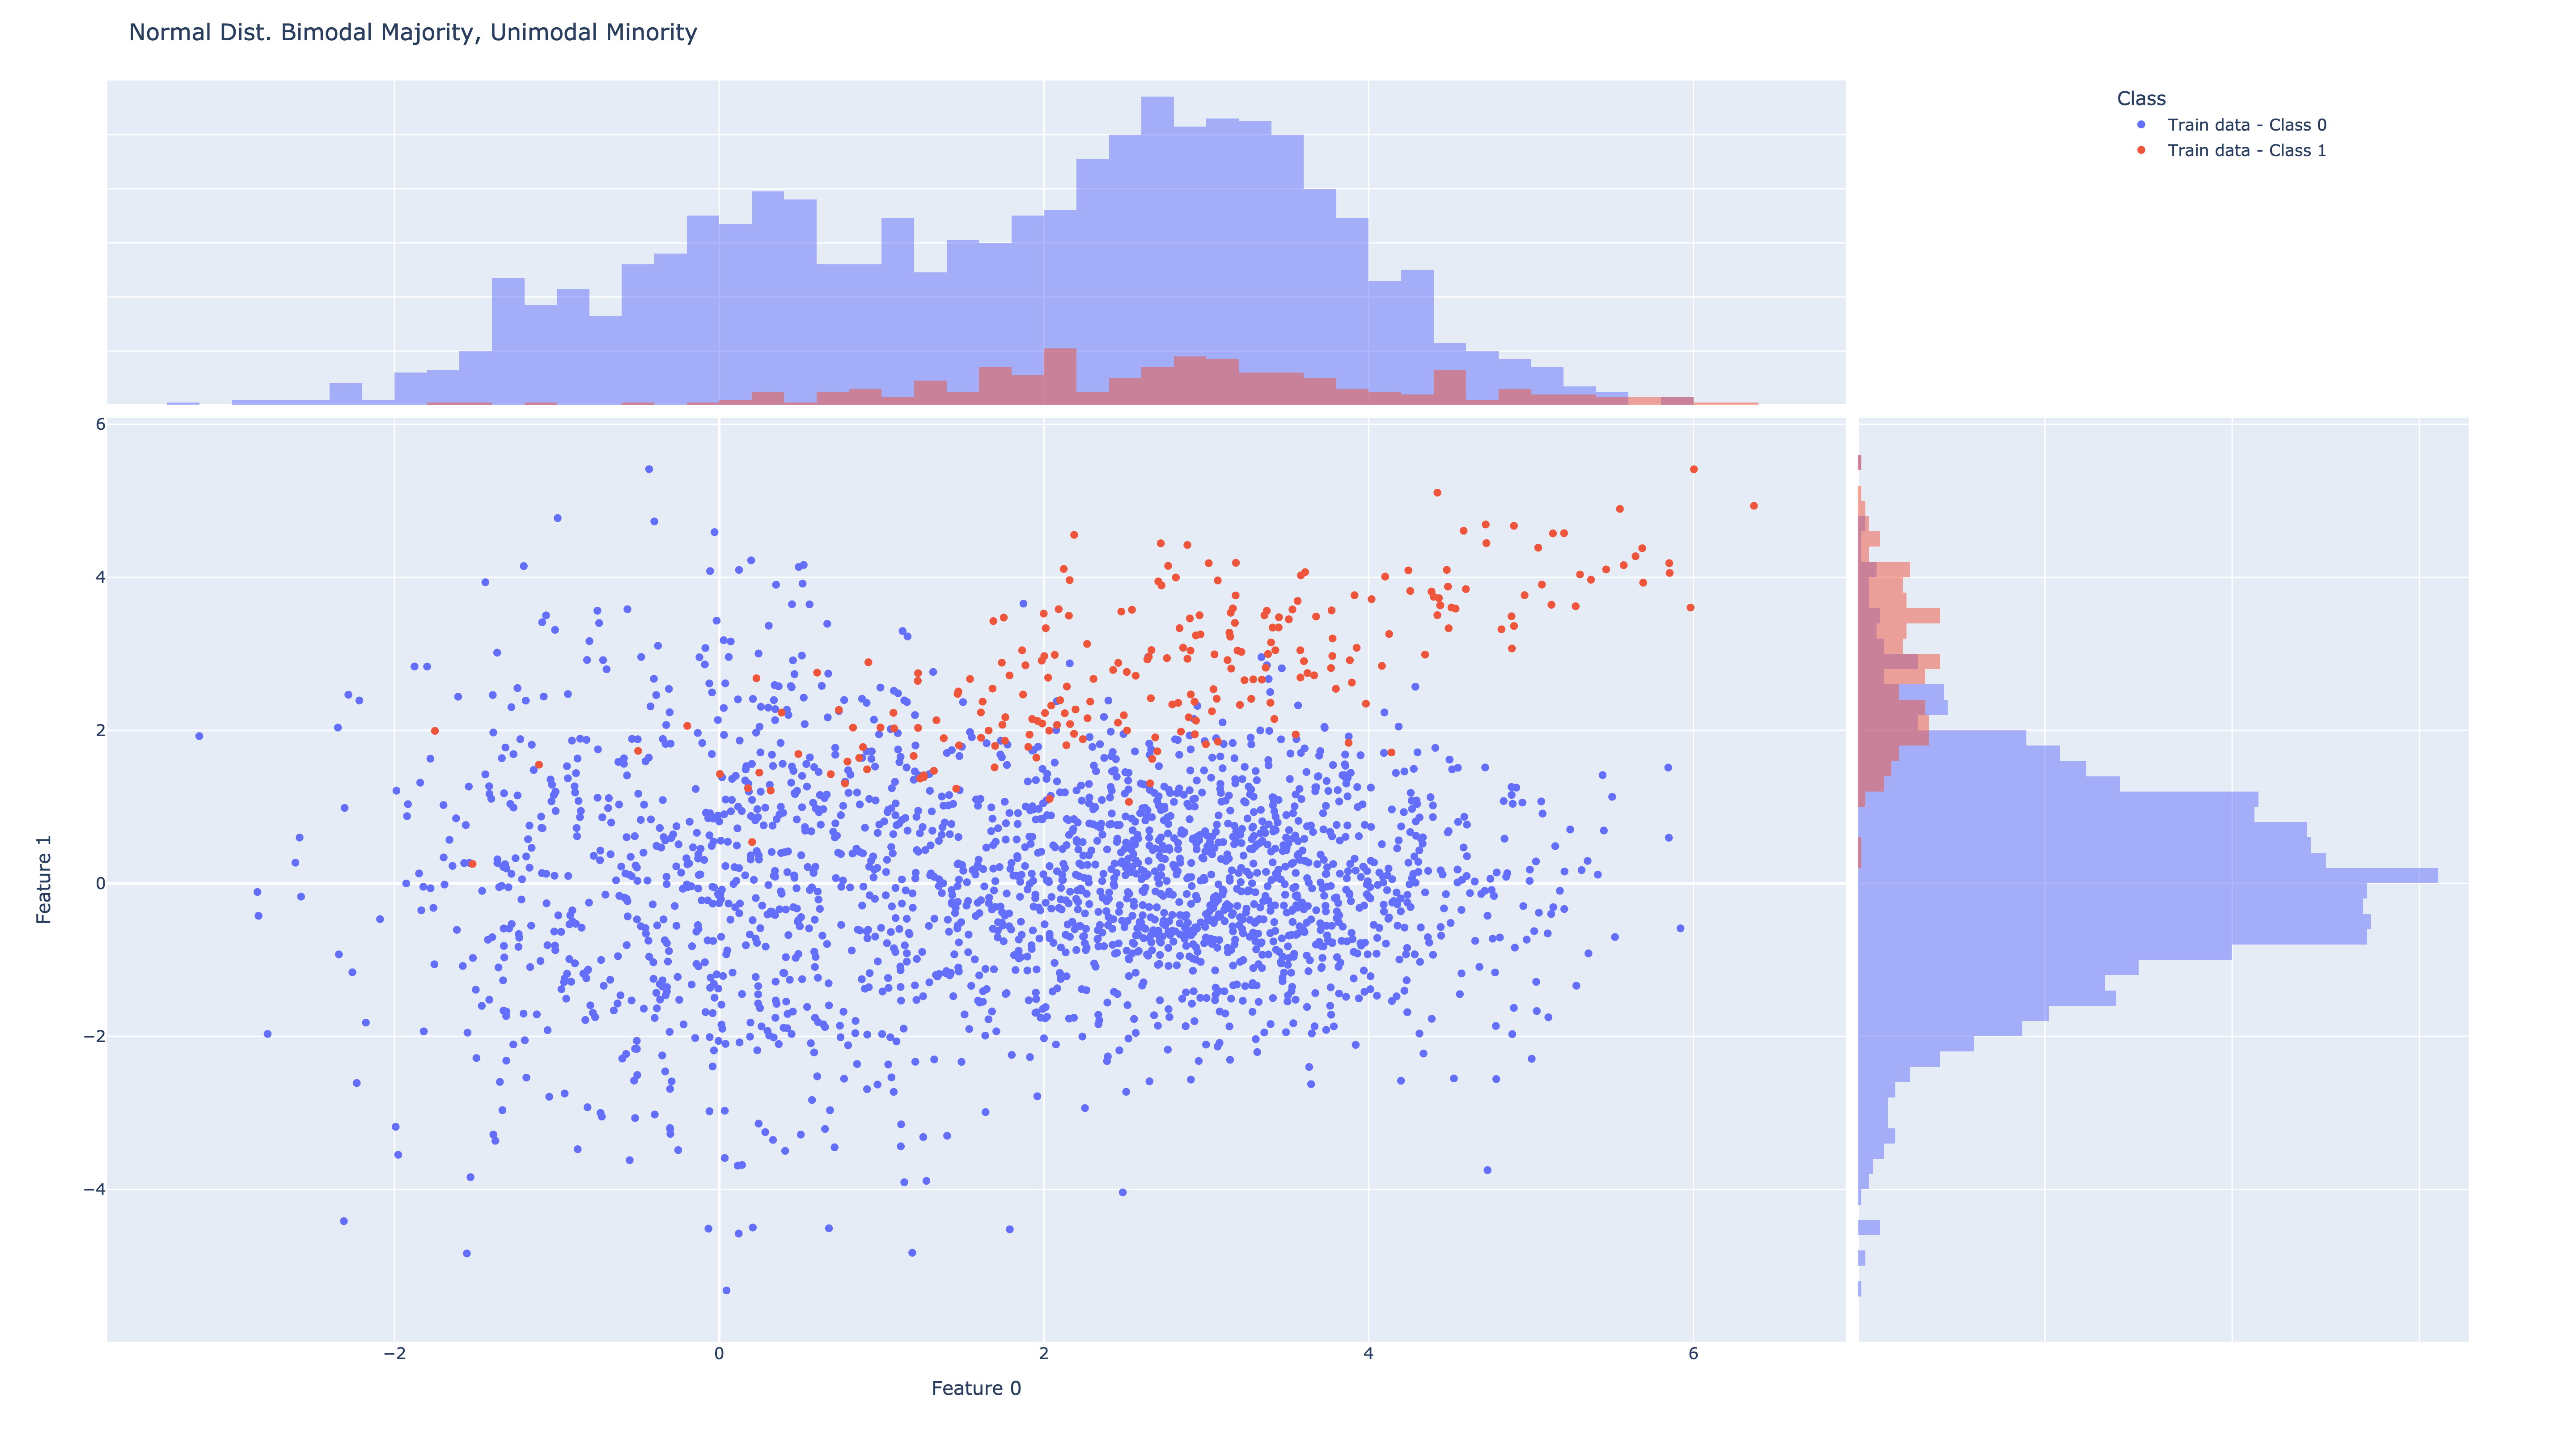
\includegraphics[width=\linewidth]{assets/data_vis/Normal_Dist_Bimodal.png}
  	\captionof{figure}{Majority bimodal, minority unimodal-normal features}
  	\label{fig:Bimodal Normal}
\end{figure}

One can see that different covariance matrices have been used 
and that a greater variety of distribution shapes and circumstances can be represented with this level of control.

The second figure comes from the same dataset, but plots feature 0 (normal) and feature 2 (beta) against each other.

\begin{figure}[H]
  	\centering
  	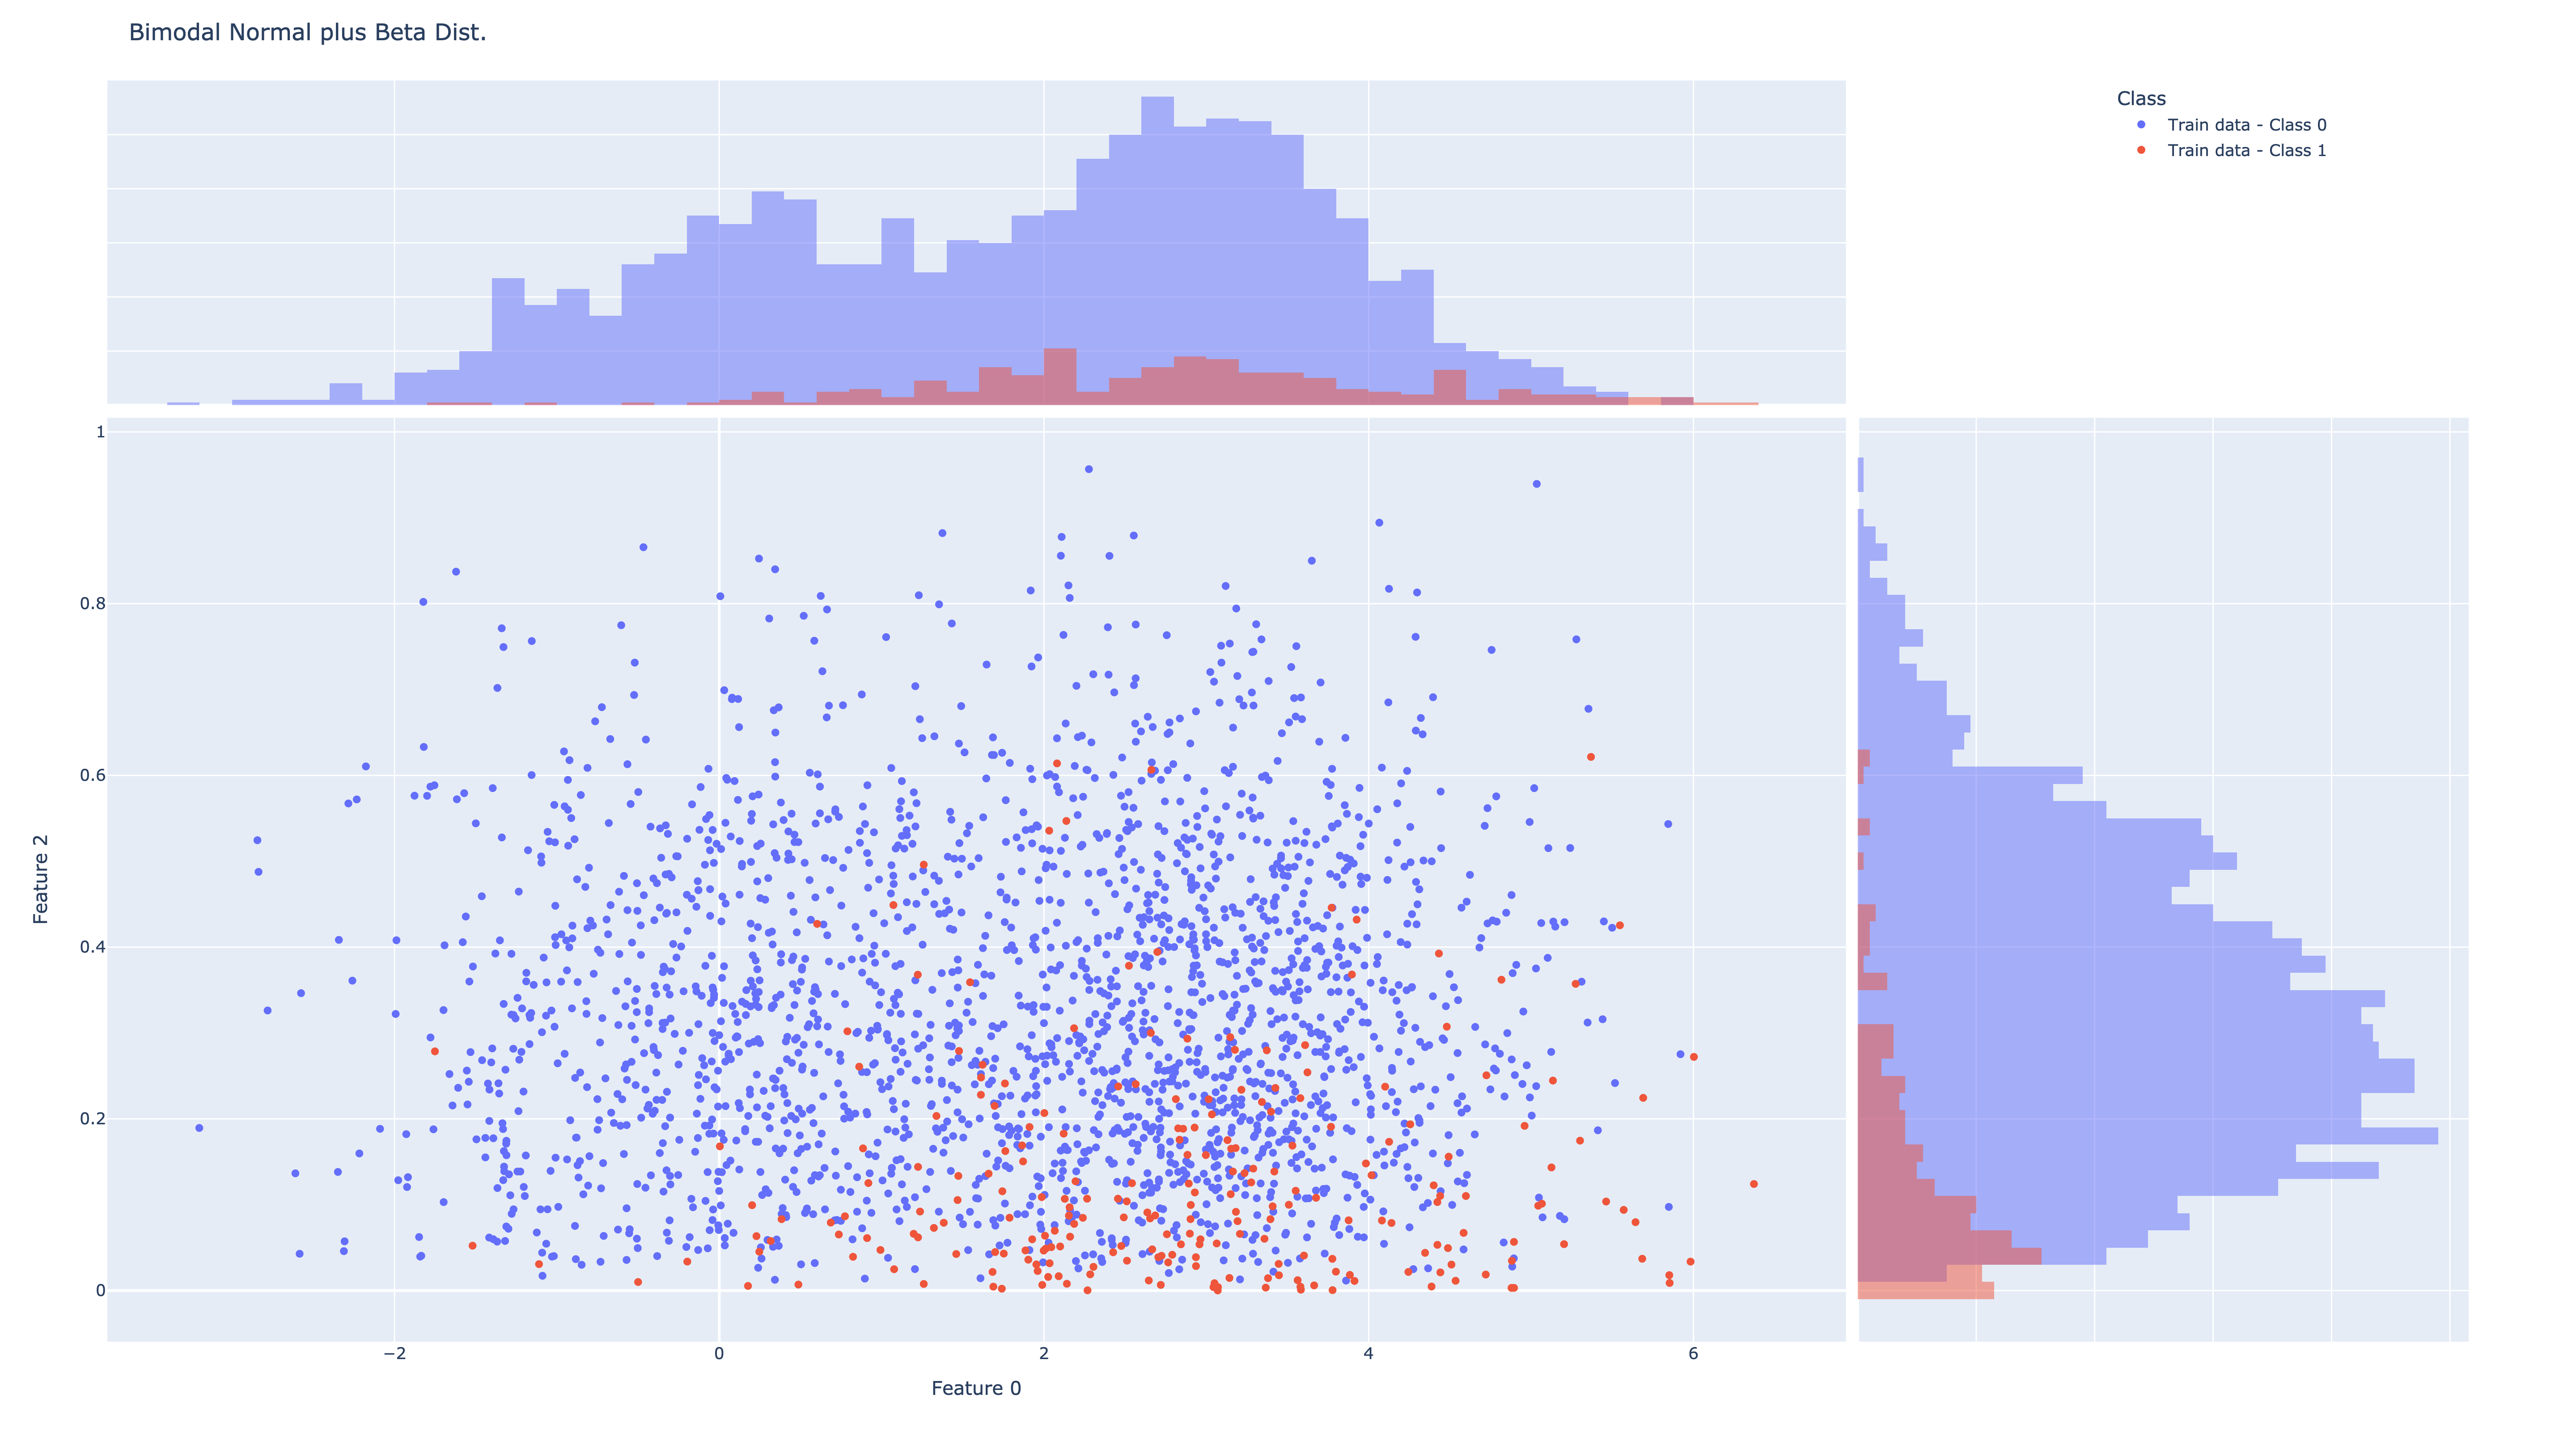
\includegraphics[width=\linewidth]{assets/data_vis/Normal_Beta.png}
  	\captionof{figure}{Bimodal-normal (0) and beta (2) features}
  	\label{fig:Normal plus Beta}
\end{figure}

%-----------------------------------------------------
\begin{comment}
\begin{figure}[H]
	\centering
	\begin{minipage}{.5\textwidth}
  		\centering
  		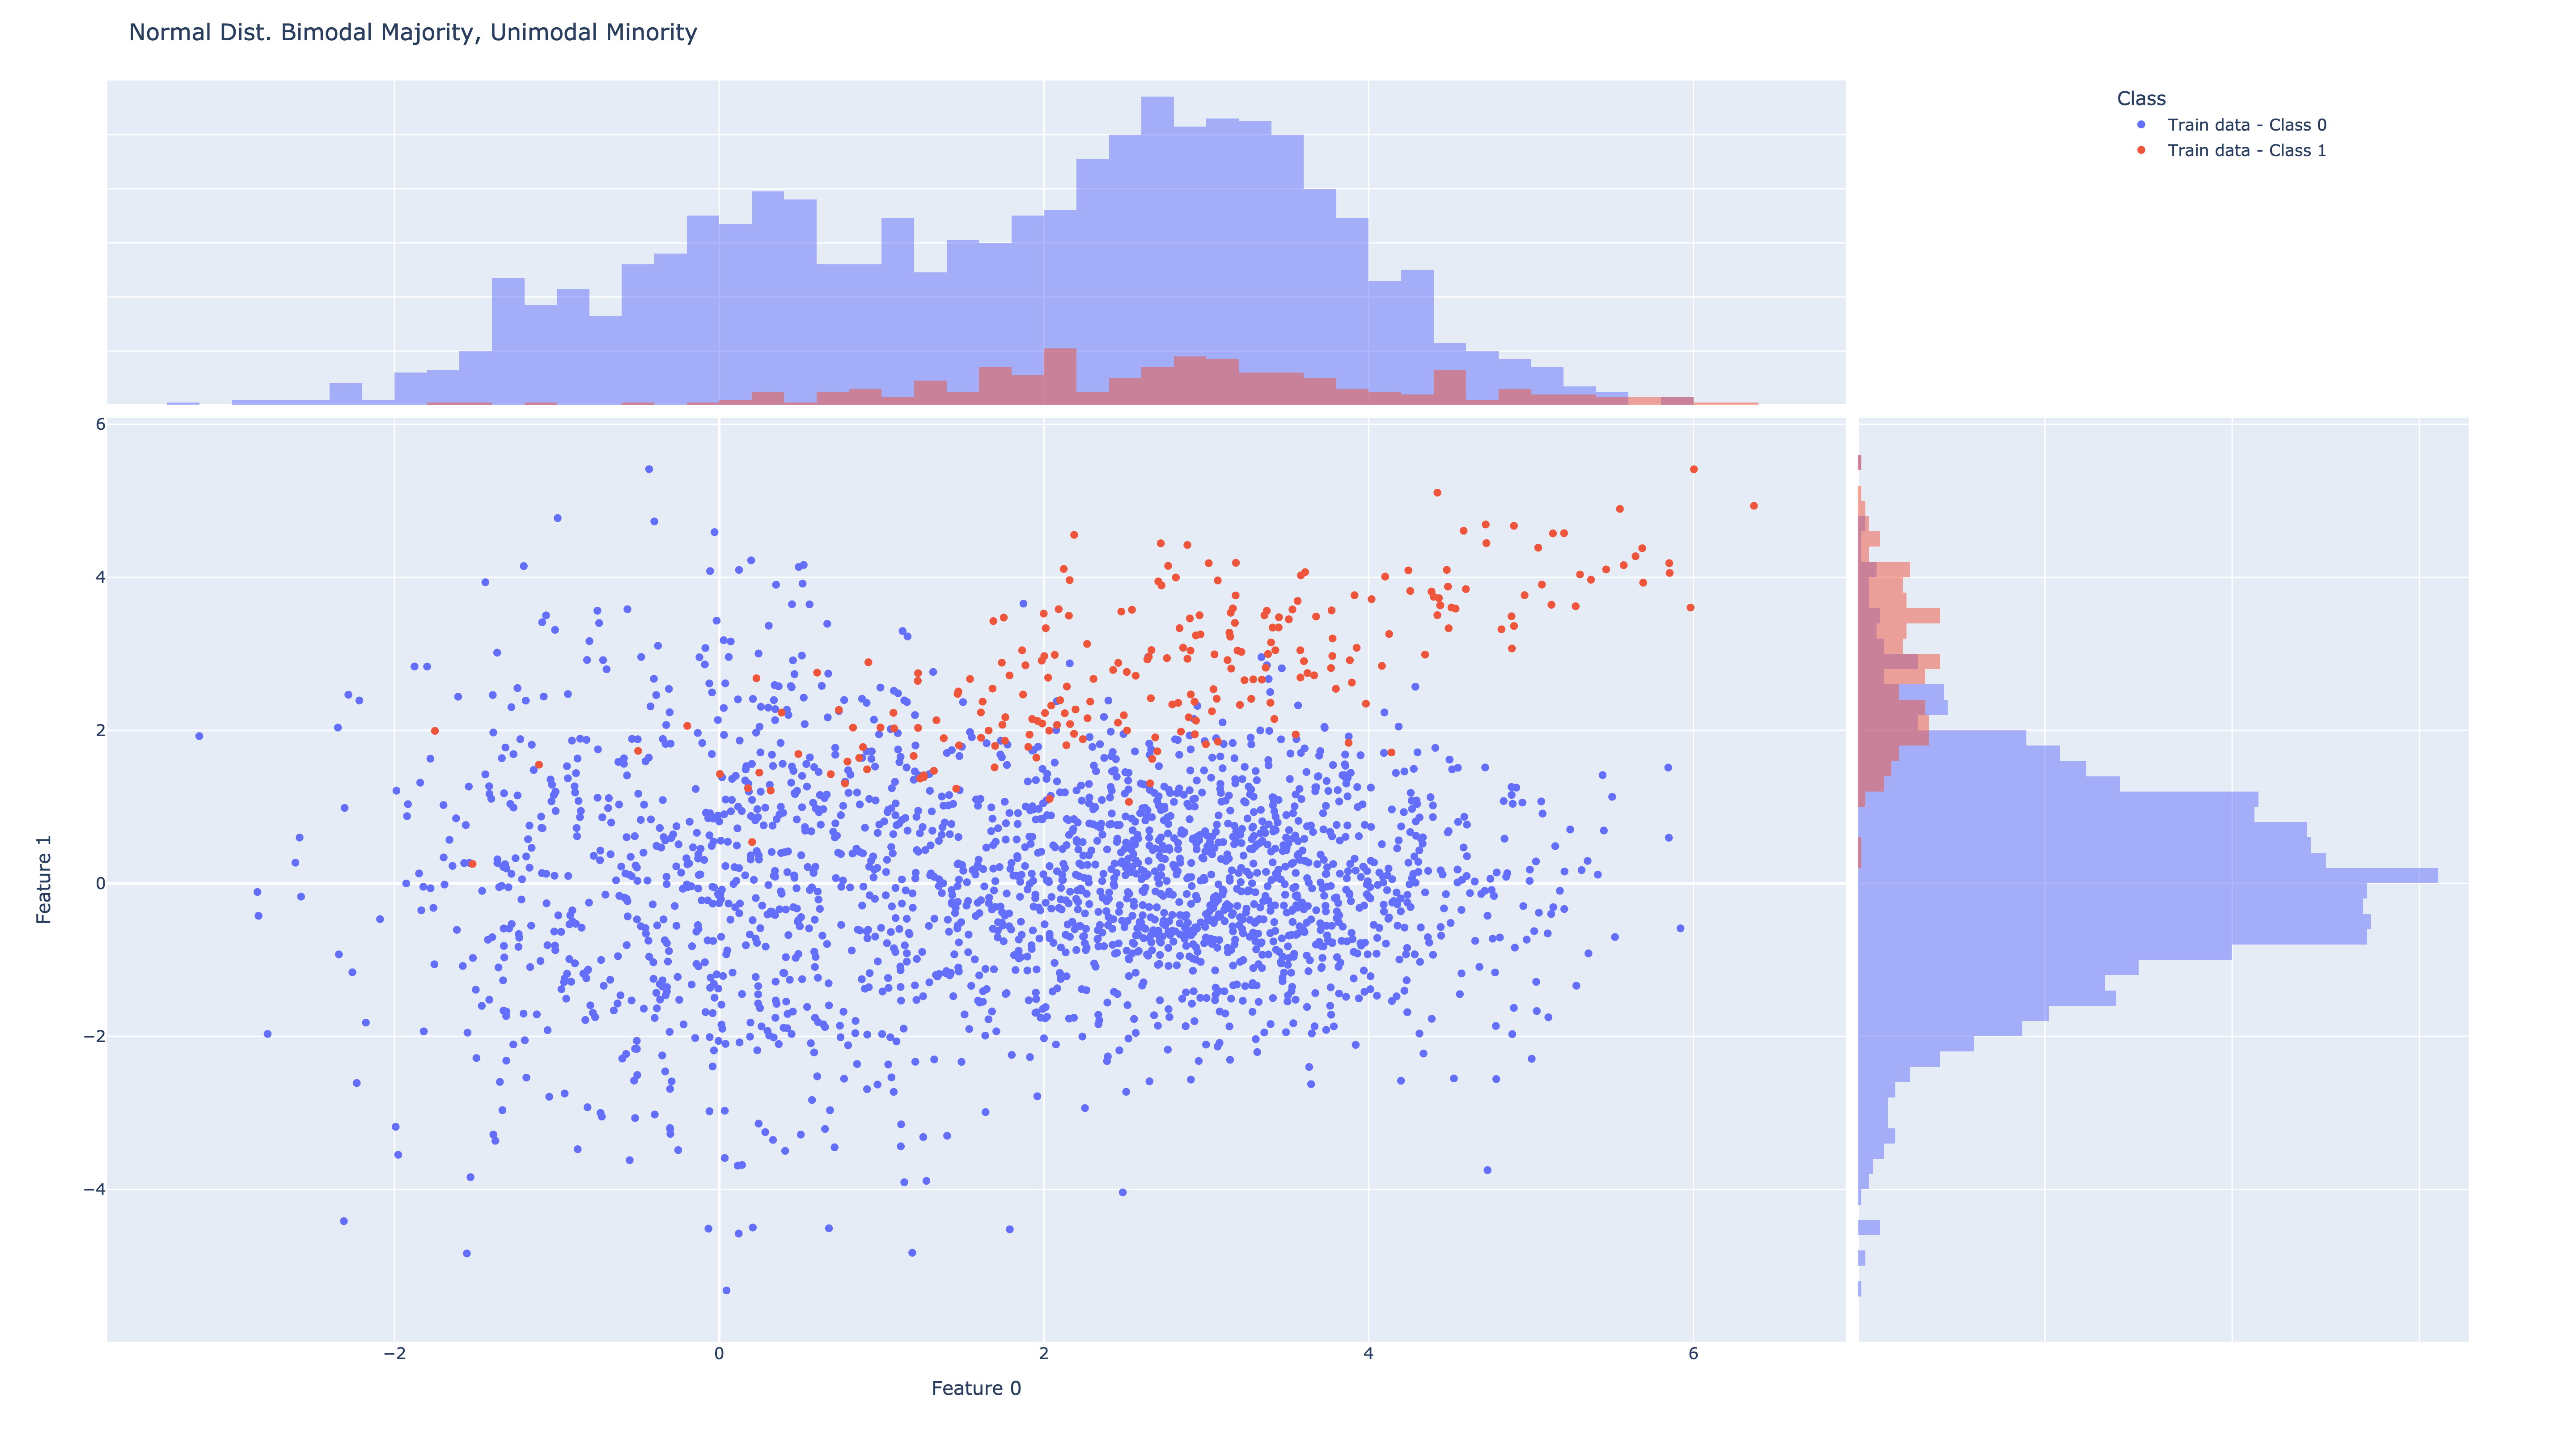
\includegraphics[width=0.98\linewidth]{assets/data_vis/Normal_Dist_Bimodal.png}
  		\captionof{figure}{Majority bimodal, minority unimodal-normal features}
  		\label{fig:Bimodal Normal}
	\end{minipage}%
	\begin{minipage}{.5\textwidth}
  		\centering
  		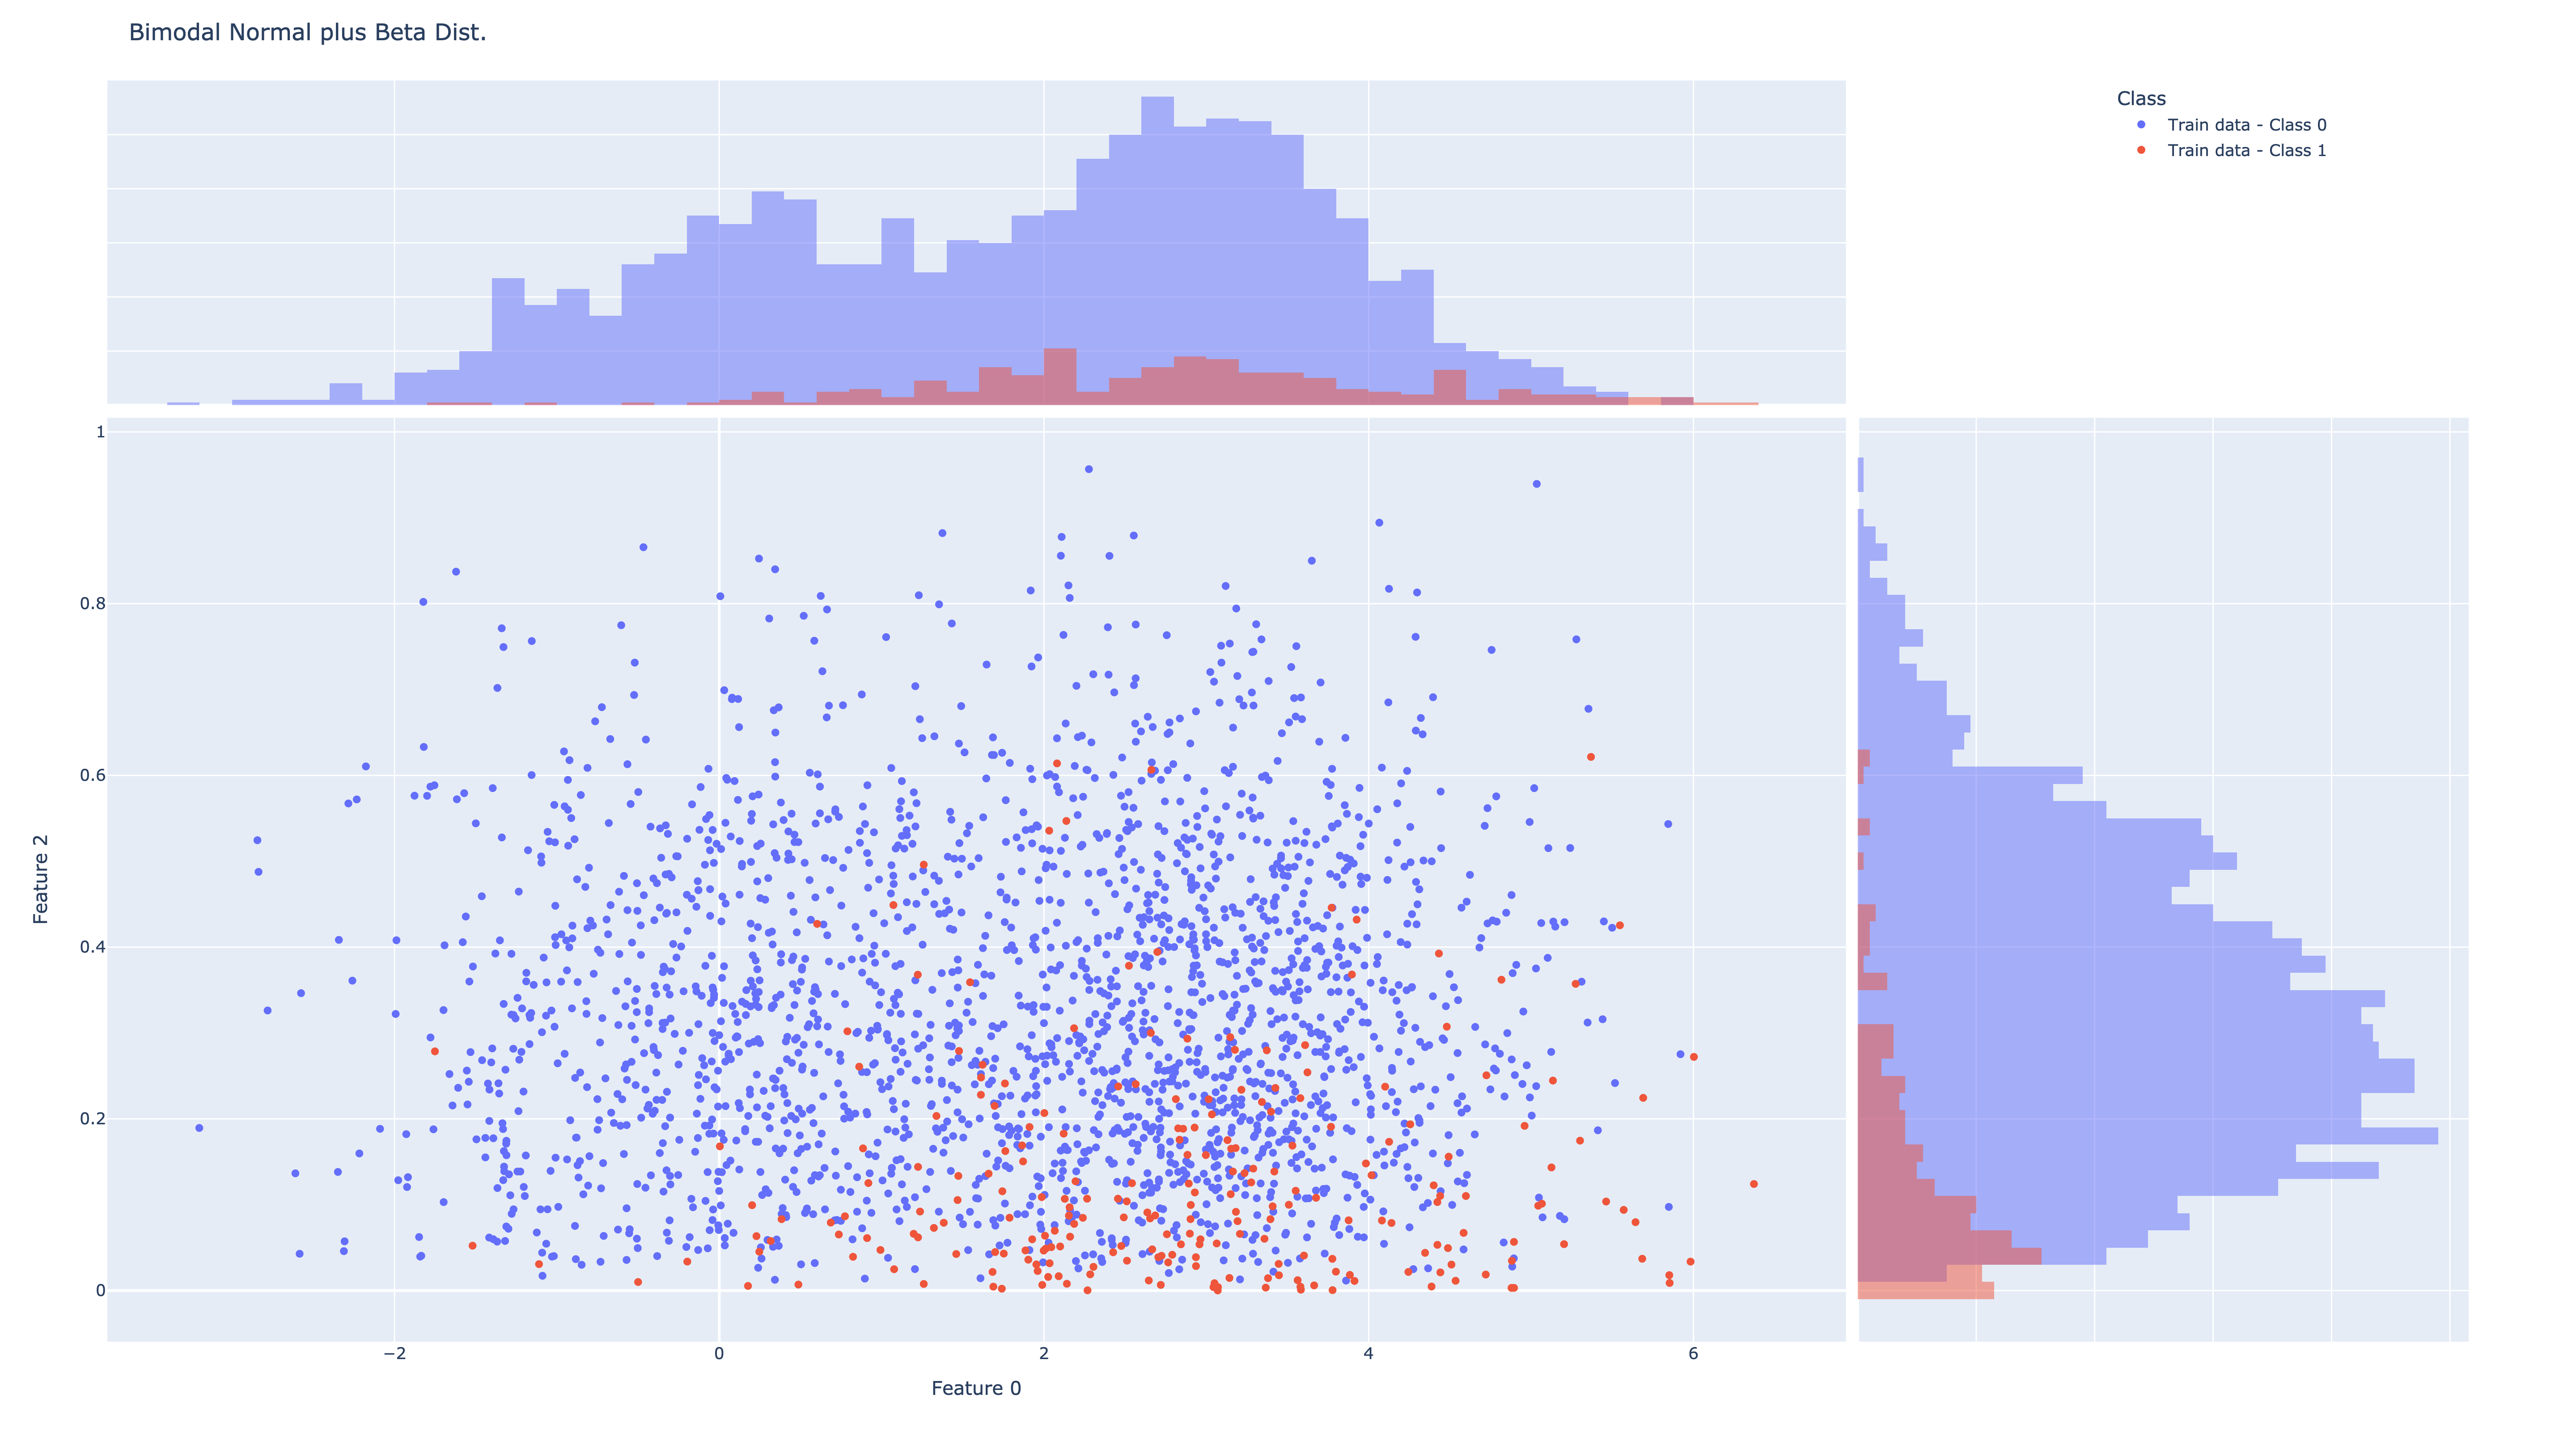
\includegraphics[width=0.98\linewidth]{assets/data_vis/Normal_Beta.png}
  		\captionof{figure}{Bimodal-normal (0) and beta (2) features}
  		\label{fig:Normal plus Beta}
	\end{minipage}
\end{figure}
\end{comment}
%-----------------------------------------------------

It is apparent that this generator allows for significantly greater flexibility but at the cost of having to specify all the parameters of every involved distribution.
This functionality made it tough to implement and somewhat tedious to use, as a test that would otherwise only require specifying a number of features or a cluster distance,
requires the user to come up with the necessary means, variances, scales or other parameters.
On the implementation side this also required to find a way to pass the parameters from a variety of distributions, keep track which parameters belonged to which feature
and re-assemble the complete feature vector before doing the train-test-split. 

The parameters used to generate the samples represented in the pictures above are given by this code:
\begin{lstlisting}[language=Python, numbers=none]
#set the parameter dictionary for the MV normal. sigma is the standard deviation
mu_c0_1 = [0,0]
mu_c0_2 = [3,0]
mu_c1 = [3,3]
sigma_c0_1 = np.array([[1,0],
                                       [0,3]])
sigma_c0_2 = np.array([[1,0],
                                       [0,1]])
sigma_c1 = np.array([[2,1],
                         		 [1,1]])
    
distributions = [st.multivariate_normal, st.beta]

#set the parameter dictionaries as a list of dictionaries with parameter dictionaries for classes individually.
dist_parameter_dicts = [
	{'modes_c0': 2,
          'modes_c1': 1,
          'mixing_weights_c0': [0.4, 0.6],
          'params_c0': {'mean': [mu_c0_1, mu_c0_2], 'cov': [sigma_c0_1, sigma_c0_2]},
          'params_c1': {'mean': [mu_c1], 'cov': [sigma_c1]}
           },
         {'modes_c0': 1,
          'modes_c1': 1,
          'params_c0': {'a': [2,3], 'b': [4,5]},
          'params_c1': {'a': [1,2], 'b': [7,8]}
           }
]

size = [2700, 300]
\end{lstlisting}

To make the number of dictionaries and sub-dictionaries one has to create smaller the list values for the distribution parameter keys 
in the \texttt{'params\_ci'} sub-dictionaries can either represent individual features or the modes of a feature of a distribution.
For example the first two features are distributed according to a multivariate normal distribution where the \texttt{'modes\_c0'} parameter specifies that the
majority class has two modes. Correspondingly the dictionary \texttt{'params\_c0'} has lists with two parameters as values that represent these modes.
For the beta distribution, from which features three and four are sampled, similar lists represent the parameters for feature three (e.g. for class 0: $a = 2, b=4$)
and feature four (again for class 0: $a = 3, b=5$) respectively.

We realise that this convention makes the dictionaries somewhat of a pain to read, however we deemed it preferable to creating still more sub-dictionaries or lengthening
the \texttt{dist\_parameter\_dicts} list, which would have made it still more convoluted to create for higher feature numbers.

Hopefully a description and seeing the code of the generator class makes the structure clear.
The initialisation method and the \texttt{create\_data} method of the generator look as follows:

\begin{lstlisting}[language=Python, numbers=none]
class Multi_Modal_Dist_Generator:
    
    def __init__(self, distributions, params_dict_list, sizes, random_state = 1234):
        self.sizes = sizes
        self.dists = distributions
        self.params_dict_list = params_dict_list
        self.random_state = random_state


    def create_data(self):
        
        self.dists_sample_lists = {'c0': [], 'c1': []}
        
        for l, parameters_dict in enumerate(self.params_dict_list):

            for i in range(2):

                if (modes:=parameters_dict[f'modes_c{i}']) > 1:
                    
                    self.create_multimodal_features(c_id = i, 
                                                    dist = self.dists[l], 
                                                    params_dict = parameters_dict[f'params_c{i}'], 
                                                    modes = modes, 
                                                    mixing_weights = parameters_dict[f'mixing_weights_c{i}'])

                else:
                    self.create_unimodal_features(c_id = i, 
                                                  dist = self.dists[l], 
                                                  params_dict = parameters_dict[f'params_c{i}'] )
        
        self.dists_sample_lists = {key: [array for array in sample_features_list]
                                   for key, sample_features_list in self.dists_sample_lists.items()}
        
        X_c0 = np.concatenate(self.dists_sample_lists['c0'], axis = 1)
        X_c1 = np.concatenate(self.dists_sample_lists['c1'], axis = 1)

        y_c0 = np.zeros(self.sizes[0])
        y_c1 = np.ones(self.sizes[1])

        self.X = np.concatenate( (X_c0, X_c1), axis = 0)
        self.y = np.concatenate( (y_c0, y_c1), axis = 0)

        # Generate a random permutation of indices
        permuted_indices = np.random.permutation(len(self.X))

        self.X = self.X[permuted_indices]
        self.y = self.y[permuted_indices]
\end{lstlisting}

Essentially the class takes a list of distributions, the sizes and a list of parameter dictionaries over which the \texttt{create\_data} method iterates.
The following process is done for each class separately, as the modes and number of samples for both classes can be different.
For each parameter dictionary the method checks whether the list of distribution parameters it contains represents the parameters of a uni- or multimodal distribution.
Depending on whether the \texttt{'modes\_ci'} parameter is greater than one or not the dictionary is passed to a different function of the class.
After the iteration the samples of each class are concatenated along the features dimension, then the samples of both classes are put together and finally they are
permuted to avoid a section-wise homogenous dataset.

The actual generation of the samples happens in the functions \texttt{create\_multimodal\_features} and \texttt{create\_unimodal\_features} shown below.

\begin{lstlisting}[language=Python, numbers=none]
    def create_multimodal_features(self, c_id, dist, params_dict, modes, mixing_weights):

        size = self.sizes[c_id]

        k = modes

        multinomial = st.multinomial(size, mixing_weights)
        comp_sizes = multinomial.rvs(size = 1)[0]

        acc_list = []

        for i in range(k):

            params = {key: value[i] for key, value in params_dict.items()}

            frozen_dist = dist(**params)

            acc_list.append(frozen_dist.rvs(size = comp_sizes[i]))

        feature_samples = np.concatenate( acc_list, axis = 0)

        feature_samples = feature_samples.reshape(size, -1)

        self.dists_sample_lists[f'c{c_id}'].append(feature_samples)
        

    def create_unimodal_features(self, c_id, dist, params_dict):

        size = self.sizes[c_id]

        k = len(next(iter(params_dict.values())))

        sample_features_list = []

        for i in range(k):

            params = {key: value[i] for key, value in params_dict.items()}

            frozen_dist = dist(**params)

            sample_features_list.append(frozen_dist.rvs(size = size))

        sample_features_list = [sample.reshape(size, -1) for sample in sample_features_list]

        self.dists_sample_lists[f'c{c_id}'].extend(sample_features_list)

\end{lstlisting}

Here the common principle is to extract the parameters of individual features or modes from the lists in the dictionary, create the distribution objects with these parameters,
and use their \texttt{.rvs} function to generate the samples.
The \texttt{create\_multimodal\_features} function is more complex and solves a problem that merits a more detailed description.
The common approach to simulate samples from a multimodal distribution is to use mixing weights for the individual components 
and sample from each component distributions according to this weight. 
A problem we needed to solve was that multiplying the desired size with the mixing weights did not guarantee an integer number of samples to sample from that component.
Rounding up or down would have altered the total number of samples in the mix and made concatenation with the other features impossible.
The solution we came up with was to introduce an additional random element and using a multinomial distribution to draw the number of samples
that each component would contribute randomly, but with a probability equal to their respective mixing weights.
This turned out to be an elegant and functional solution that represents the mixing components fairly accurately, especially for large sample sizes. \\

In order to use this generator we created a second version of the pipeline. 
This version differs little from the first approach in principle but has significantly more complicated code as we experimented with the idea of localising iteration, 
that we had previously done with additional for-loops, to the dedicated classes in the hope of greater efficiency due to less need to pass datasets and recreate instances.
So for example, instead of initialising the classifier class for each classifier individually this version initialises the \texttt{DictIterClassifier} with all used classifiers at once.
As the approach didn't significantly improve computational performance and was superseded by the FMLP approach described in the next chapter
we just representatively show the \texttt{DictIterClassifier} here.

\begin{lstlisting}[language=Python, numbers=none]
class DictIterClassifier(BaseEstimator, ClassifierMixin):

    def __init__(self, classifiers_dict = {}, classifier_params = {'random_state': 42}):

        classifier_list = [(name, classifier) for name, classifier in classifiers_dict.items()]

        if not isinstance(classifier_params, list):
            self.classifier_params = [classifier_params for _ in range(len(classifier_list))]
        else:
            self.classifier_params = classifier_params

        self.classifier_dict_list = [{'name': name, 'classifier': classifier(**params)}
                                      for (name, classifier), params in zip(classifier_list, self.classifier_params)]


    def fit(self, X, y):
        
        self.classifiers_dict_list = [
            {**dict, 'classifier': dict['classifier'].fit(X,y)} 
            for dict in self.classifier_dict_list
        ]
        return self
    

    def predict(self, X):
            
        predictions_dict_list = [
            dict(
                 {key: val for key,val in clsf_dict.items() if key != 'classifier'},
                 **{
                     'predicted_proba': clsf_dict['classifier'].predict_proba(X),
                     'predicted_y': clsf_dict['classifier'].predict(X),
                     'classes': clsf_dict['classifier'].classes_
                    }
            )
            for clsf_dict in self.classifier_dict_list
        ]
        
        return predictions_dict_list
        
\end{lstlisting}

While this pipeline approach didn't reap significant benefits compared to the original version, apart from functioning with the new generator, 
the elaborate transformations of and iterations over compositions of lists and dictionaries proved very helpful in the design of the FMLP approach.

\subsection{Fast Pipeline Approach (FMLP)}

Conducting an experiment with the two previous versions of the pipeline involves concatenated for-loop iterations over the respective parameter sets.
At each step of an iteration the data is passed between the active class instances of the pipeline and subsequently stored as an instance attribute before transformation.
There are two main sources of overhead that these approaches incur due to these operations.
For one, every iteration involves the creation and subsequent destruction of large arrays in memory, 
and while \texttt{numpy}'s C implementation guarantees efficient calculations on arrays of fixed size, 
creation of these arrays incurs significant overhead as large contiguous blocks of memory have to be reserved and released.
Secondly, at each step of an iteration the data is passed, i.e. copied, 
between the individual pipeline components, which again incurs the overhead due to creation and garbage collection.

The key idea of the last pipeline approach is to reduce the impact of these sources of overhead by creating large \texttt{numpy} arrays of adequate dimensions once,
giving each component of the pipeline a reference to the data instead of a copy, and applying the algorithms directly to sections of these large arrays.

To this end we introduce an intermediate parent class which only has an empty dictionary as a class attribute:
\begin{lstlisting}[language=Python, numbers=none]
class Data():

    	data_dict = {}
\end{lstlisting}

The other classes inherit from \texttt{Data} and modify the contents of the \texttt{data\_dict} dictionary.
To direct this process and create the necessary \texttt{numpy} arrays we created the \texttt{Assessor} class.
The \texttt{Assessor} takes in the \texttt{test\_size}, a list of dictionaries for the generator, and as before, a dictionary each for the balancers and classifiers to be used.
Its \texttt{\_\_init\_\_} method looks like this

\begin{lstlisting}[language=Python, numbers=none]
class Assessor(Data):

    def __init__(self, test_size, generation_dict_list, balancers_dict, classifiers_dict):

        Data.data_dict = {}

        self.test_size = test_size
        self.generation_dict_list = generation_dict_list

        balancer_list = [(name, balancer) for name, balancer in balancers_dict.items()]
        
        clsf_list = [(name, classifier) for name, classifier in classifiers_dict.items()]

        self.exp_dim = (len(generation_dict_list), len(balancers_dict), len(classifiers_dict))
        
        self.data_dict['assignment_dict'] = {(a, b, c): [gen_dict, bal, clsf]
                                             for (a, gen_dict), (b, bal), (c, clsf)
                                             in product(enumerate(generation_dict_list), 
                                                        enumerate(balancer_list), 
                                                        enumerate(clsf_list)
                                                        )
                                            }

\end{lstlisting}

Here the baseline dimensions for the \texttt{numpy} arrays that are to be created are calculated and saved in \texttt{self.exp\_dim} and 
the generation dictionaries and the names and classes corresponding to the balancers and classifiers are stored in the \texttt{assignment\_dict} 
under a three dimensional tuple key. 
This dictionary is essential to assign the methods to the correct positions in the later steps and the correct labels in the output files.

After initialisation the following methods are to be called in sequence if one wishes to execute the pipeline. 
In the generation function below we first check for the largest number of samples and dimensions to accommodate, 
then four \texttt{numpy} arrays of that size are created and filled with\texttt{np.nan} values.
Subsequently we iterate over the generation dictionaries in the stored list and assign a generation index to place the generated data in the correct part of the raw data arrays.
For each generation dictionary the \texttt{FMLP\_Generator} class is instantiated and its \texttt{prepare\_data} method is executed.
\begin{lstlisting}[language=Python, numbers=none]
def generate(self):     

	test_size = self.test_size
	table_infos = [extract_table_info(generation_dict) for generation_dict in self.generation_dict_list]
	
	self.d = max([info[0] for info in table_infos])
	n = max([info[1] for info in table_infos])
	a = self.exp_dim[0]
	        
	trainset_size = int((1-test_size)*n)
	testset_size = int(test_size*n)
	
	self.data_dict['org_X_train'] = np.full(shape = (a, trainset_size, self.d), fill_value = np.nan)
	self.data_dict['org_y_train'] = np.full(shape = (a, trainset_size,), fill_value = np.nan)
	
	self.data_dict['org_X_test'] = np.full(shape = (a, testset_size, self.d), fill_value = np.nan)
	self.data_dict['org_y_test'] = np.full(shape = (a, testset_size,), fill_value = np.nan)
	
	for i, generation_dict in enumerate(self.generation_dict_list):
		generation_dict['gen_index'] = i
		generator = FMLP_Generator(**generation_dict)
		generator.prepare_data(self.test_size)
\end{lstlisting}

The \texttt{FMLP\_Generator} doesn't differ much from the generator in the previous section apart from inheriting from \texttt{Data} and the \texttt{prepare\_data} method,
which now doesn't return the split raw data but instead inscribes it in the data arrays instantiated earlier.

The next method in line is the \texttt{balance} method. It is called with \texttt{bal\_params\_dicts} as a parameter that defaults to an empty dictionary.
This parameter is supposed to be a dictionary of dictionaries where each key should be a balancers name and the corresponding value should be a dictionary 
that contains the instantiation parameters of the balancer, most importantly the \texttt{'sampling\_strategy'}.

\begin{lstlisting}[language=Python, numbers=none]
    def balance(self, bal_params_dicts = {}):

        a, b, c = self.exp_dim
        y_train = self.data_dict['org_y_train']

        default_strategy = 'auto'
        max_c1 = max([np.sum(y_train[data_ind] == 1) for data_ind in range(a)])
        max_total_samples = 0

        for data_ind in range(a):
            #check if a balancer parameter dict is given
            if bal_params_dicts:
                #iterate over the parameter dictionaries that are given
                for bal_dict in bal_params_dicts.values():

                    max_total_samples = max(max_total_samples, sum(calculate_no_samples(y_train[data_ind], bal_dict['sampling_strategy']).values()))

            #compare to default strategy if not every balancer has a dict
            if len(bal_params_dicts) < b:
                max_total_samples = max(max_total_samples, sum(calculate_no_samples(y_train[data_ind], default_strategy).values()))
        
        k = max_c1 + max_total_samples

        self.data_dict['bal_X_train'] = np.full(shape = (a, b, k, self.d), fill_value = np.nan)
        self.data_dict['bal_y_train'] = np.full(shape = (a, b, k, ), fill_value = np.nan)

        data_balancer = FMLP_DataBalancer(bal_params_dicts)
        
        data_balancer.balance_data()
\end{lstlisting}

The most complicated part of this step was to find the maximal number of samples for which to reserve space in the balanced data arrays.
\texttt{Imblearn} balancers allow a wide range of options to set the \texttt{'sampling\_strategy'} and depending on which strategy the user settles on,
the final amount of samples varies drastically. This approach to the pipeline in general sacrifices memory consumption for faster execution time, 
but optimally the created arrays should not be much larger than they have to be to accommodate the data. 
To achieve an array that is as small as possible but as large as necessary the \texttt{calculate\_no\_samples} function calculates the number of samples
that can be expected depending on the sampling strategy and uses the maximum number among all balancers and datasets to be balanced.

The instantiation of the balancers and the iteration is happening completely in the realm of the \texttt{FMLP\_DataBalancer} class. 
This is unlike the generation step where the iteration is in the \texttt{generate} method where a new class instance of the generator was created at each iteration.
Adding a serialised iteration functionality to the generator would have been considerably more effort to implement as the class already has a high degree of complexity,
hence we decided to go for the simpler approach there. For \texttt{FMLP\_DataBalancer} however it was possible to do the iterations in an elegant way.

Upon initialisation the class creates a sub-dictionary of the \texttt{assignment\_dict}, dropping the index for the classifier in the keys,
and the generator dictionaries and classifier pairs, keeping only name and class of the balancers.
The class also stores a dictionary for the parameters of the balancers which is composed of those parameter dictionaries the user specified in the function call
and a default dictionary with \texttt{'sampling\_strategy' : 'auto'} for those balancers without specification.

\begin{lstlisting}[language=Python, numbers=none]
class FMLP_DataBalancer(Data):

    def __init__(self, bal_params_dict = {}):

        self.balancer_dict = {(i,j): assign_list[1] for (i,j,k), assign_list in self.data_dict['assignment_dict'].items()}
        
        default_dict = {'sampling_strategy': 'auto', 'random_state': 42}
        self.bal_params_dict = {name: bal_params_dict[name]
                                if name in bal_params_dict else default_dict
                                for (name, bal) in self.balancer_dict.values()}
        
     
    def balance_data(self):

        X = self.data_dict['org_X_train']
        y = self.data_dict['org_y_train']

        for (data_ind, bal_ind), (name, balancer) in self.balancer_dict.items():

            X_bal = X[data_ind]
            y_bal = y[data_ind]
            
            # Drop rows with NaN values
            X_bal = X_bal[~np.isnan(X_bal).all(axis = 1)]
            # Drop columns with NaN values
            X_bal = X_bal[: , ~np.isnan(X_bal).all(axis = 0)]
            y_bal = y_bal[~np.isnan(y_bal)]
            
            if balancer == None:
                resample = (X_bal,y_bal)

            else:
                balancer = balancer(**self.bal_params_dict[name])
                resample = balancer.fit_resample(X_bal, y_bal)

            n, d = np.shape(resample[0])
                        
            self.data_dict['bal_X_train'][data_ind, bal_ind, :n, :d] = resample[0]
            self.data_dict['bal_y_train'][data_ind, bal_ind, :n] = resample[1]
            
\end{lstlisting}

The \texttt{balance\_data} method retrieves the raw training data from the dedicated arrays and iterates over the reduced tuple indices from the \texttt{balancer\_dict}.
For each combination of balancer and dataset the not-NaN part of the corresponding sub-array of the raw data is selected and new samples are created. 
The resulting samples are placed in their respective positions in the balancer data array created by the \texttt{Assessor}.

The classification and prediction steps follow the same general dynamic, although made somewhat simpler as the appropriate array size is already known.
One array is created for the predictions on the test set, another for predicted probabilities on the test set and a final one that stores the class order.
 
\begin{lstlisting}[language=Python, numbers=none]
    def clsf_pred(self):

        a, n = np.shape(self.data_dict['org_y_test'])

        self.data_dict['clsf_predictions_y'] = np.full(shape = self.exp_dim + (n,), fill_value = np.nan)
        self.data_dict['clsf_predictions_proba'] = np.full(shape = self.exp_dim + (n, 2), fill_value = np.nan)
        self.data_dict['classes_order'] = np.full(shape = self.exp_dim + (2,), fill_value = np.nan)

        data_classifier = FMLP_DataClassifier()

        data_classifier.fit()

        data_classifier.predict()

\end{lstlisting}

Storing the order is necessary as for a \texttt{scikit-learn} classifier the predicted probabilities are ordered by the sequence in which the classes appeared in the training set,
which we cannot anticipate due to the randomness in generation. 
The initialisation method of \texttt{FMLP\_DataClassifier} follows the same procedure as we already detailed for the \texttt{FMLP\_DataBalancer}.
Also the remaining two methods follow similar steps. 
In both the \texttt{fit} and the \texttt{predict} method the iteration proceeds over a transformed version of the \texttt{assignment\_dict} 
where only the classifier entries were selected and their classes instantiated.

\begin{lstlisting}[language=Python, numbers=none]
class FMLP_DataClassifier(Data):

    def __init__(self, clsf_params_dict = {}):

        default_dict = {'random_state': 42}
        classifier_dict = {key: assign_list[2] for key, assign_list in self.data_dict['assignment_dict'].items()}
        
        classifier_dict = {key: (name, clsf(**clsf_params_dict[name]))
                           if name in clsf_params_dict else (name, clsf(**default_dict))
                           for key, (name, clsf) in classifier_dict.items()}
        
        self.classifier_dict = classifier_dict


    def fit(self):

        X = self.data_dict['bal_X_train']
        y = self.data_dict['bal_y_train']
        
        for (i,j,k), (name, clsf) in self.classifier_dict.items():
            
            X_fit = X[i, j, :, :]
            y_fit = y[i, j, :]

            # Drop rows with NaN values
            X_fit = X_fit[~np.isnan(X_fit).all(axis = 1)]
            # Drop columns with NaN values
            X_fit = X_fit[: , ~np.isnan(X_fit).all(axis = 0)]
            
            y_fit = y_fit[~np.isnan(y_fit)]
            
            self.classifier_dict[(i,j,k)] = (name, clsf.fit(X_fit, y_fit))

        return self
    

    def predict(self):

        X = self.data_dict['org_X_test']

        for (i,j,k), (name, clsf) in self.classifier_dict.items():
            
            X_test = X[i, :, :]

            # Drop rows with NaN values
            X_test = X_test[~np.isnan(X_test).all(axis = 1)]
            # Drop columns with NaN values
            X_test = X_test[: , ~np.isnan(X_test).all(axis = 0)]

            n_i = len(X_test)

            self.data_dict['clsf_predictions_y'][i, j, k, : n_i] = clsf.predict(X_test)
            self.data_dict['clsf_predictions_proba'][i, j, k, : n_i, :] = clsf.predict_proba(X_test) 
            self.data_dict['classes_order'][i, j, k, :] = clsf.classes_

\end{lstlisting}

Every dataset-balancer-classifier combination in this tensor is then first \texttt{fit} with the balanced data, corresponding to the position in the tensor, 
and then called on to give predictions in \texttt{predict}. Each time we select a view of the whole data we drop the NaN components from the view before passing it.

The next step to achieve a similar functionality as the previous pipeline versions was to calculate the standard metrics. 
Once one has understood the design of the previous functions in \texttt{Assessor} this one is straightforward to understand due to the similarity.
The user passes a dictionary of named standard metric-functions. 
'Standard' here essentially refers both to the commonality of the metrics as well as the technical aspect of their calculation:
Only the original test sets and the trained classifiers predictions on them are necessary.
Should the user not pass a dictionary with the desired standard metrics a default will be used. We applied this default to the majority of our tests.

\begin{lstlisting}[language=Python, numbers=none]

    def calc_std_metrics(self, std_metrics_dict = {}):

        default_metrics = {
            'accuracy': accuracy_score,
            'precision': precision_score,
            'recall': recall_score,
            'F1 score': f1_score,
            'ROC AUC Score': roc_auc_score,
        }

        metrics_dict = std_metrics_dict or default_metrics


        self.data_dict['std_metrics_res'] = np.full(shape = self.exp_dim + (len(metrics_dict),), fill_value = np.nan)
        
        metrics = FMLP_Metrics(metrics_dict)

        metrics.confusion_metrics()

        std_metrics_res = self.data_dict['std_metrics_res'].reshape(-1, len(metrics_dict))

        results_df = pd.DataFrame(std_metrics_res, columns= [name for (name, metr_func) in metrics.std_metric_list])

        reference_list = [self.data_dict['assignment_dict'][(i, j, k)] 
                          for i in range(self.exp_dim[0]) 
                          for j in range(self.exp_dim[1]) 
                          for k in range(self.exp_dim[2])]

        reference_list = [extract_table_info(alist[0])+[alist[1][0], alist[2][0]] for alist in reference_list]

        reference_df = pd.DataFrame(reference_list, columns= ['n_features', 
                                                              'n_samples', 
                                                              'class_ratio', 
                                                              'distributions', 
                                                              'balancer', 
                                                              'classifier'])

        results_df = pd.concat([reference_df, results_df], axis = 1)

        return results_df
\end{lstlisting}

What is different in this part of the pipeline is that the names and the crude information from the generator dictionaries contained in the \texttt{assignment\_dict}
is transformed into a reference list that we use to create the \texttt{results\_df}.
The \texttt{FMLP\_Metrics} classes \texttt{confusion\_metrics} function is so similar in structure to the functions previously described 
that we will just show the code without additional explanation:

\begin{lstlisting}[language=Python, numbers=none]
def confusion_metrics(self):
	
        y_test = self.data_dict['org_y_test']
        y_pred = self.data_dict['clsf_predictions_y']

        for (i,j,k) in self.data_dict['assignment_dict']:
            
            y_i_test = y_test[i]
            y_i_test = y_i_test[~np.isnan(y_i_test)]

            y_clsf_pred = y_pred[i, j, k]
            y_clsf_pred = y_clsf_pred[~np.isnan(y_clsf_pred)]

            evaluation = np.array([metr_func(y_i_test, y_clsf_pred) for (name, metr_func) in self.std_metric_list])

            self.data_dict['std_metrics_res'][i, j, k, :] = evaluation
\end{lstlisting}


\subsection{Discussion}

The greatest challenge overall in the creation of these pipelines was the administration of parameters. 
Allowing all segments of the pipeline to be general enough to accept the large variety of parameters that generator, balancers and classifiers possess,
while maintaining usability and a streamlined workflow, was very difficult.
We wanted the pipeline to be as general as possible to enable a large body of experiments to be conductable but assure that a user does not have to provide
all the parameters in a short experiment.

As mentioned before the FMLP approach will on average be faster but as it stores large arrays in memory that remain throughout the execution of the pipeline,
it places a much heavier burden on available RAM memory. 
While we did not have the time to implement this here, the computational efficiency of this approach could be greatly increased still 
with the use of parallel processing and GPU recruitment. 
Furthermore one could create custom versions of the \texttt{imblearn} balancing algorithms and \texttt{scikit-learn} classifiers that sacrifice some generality
in favour of efficient serialisation that makes greater use of the optimised matrix operations of modern GPUs.
The FMLP approach allows to test various balancers and classifiers with the freedom to set all parameters for each of them.
It does not however enable serialised experiments where different parameter sets are passed to the same balancer or classifier without additional exterior iteration.





%\subsection{Pipeline description}


